\documentclass[format=acmsmall, review=false, screen=true]{acmart}

\usepackage{booktabs} % For formal tables

\usepackage[ruled]{algorithm2e} % For algorithms
\renewcommand{\algorithmcfname}{ALGORITHM}
\SetAlFnt{\small}
\SetAlCapFnt{\small}
\SetAlCapNameFnt{\small}
\SetAlCapHSkip{0pt}
\IncMargin{-\parindent}
\graphicspath{ {images/} }


% Metadata Information
\acmJournal{TWEB}
\acmVolume{0}
\acmNumber{4}
\acmArticle{00}
\acmYear{2017}
\acmMonth{3}
\copyrightyear{2017}
\acmArticleSeq{0}

% Copyright
%\setcopyright{acmcopyright}
\setcopyright{acmlicensed}
%\setcopyright{rightsretained}
%\setcopyright{usgov}
%\setcopyright{usgovmixed}
%\setcopyright{cagov}
%\setcopyright{cagovmixed}

% DOI
\acmDOI{0000001.0000001}

% Paper history
\received{March 2017}
\received[revised]{March 2017}
\received[accepted]{March 2017}


% Document starts
\begin{document}
\title{Report for Multithreaded Web server}  
\author{Hassaan Fayyaz Ahmed}
%\orcid{1234-5678-9012-3456}
\affiliation{%
  \institution{Lahore University of Management Sciences}
  \streetaddress{Opposite Sector U, DHA}
  \city{Lahore}
  \state{Punjab}
  \postcode{54810}
  \country{Pakistan}}
\author{Muhammad Qasim Hunain}
%\orcid{1234-5678-9012-3456}
\affiliation{%
  \institution{Lahore University of Management Sciences}
  \streetaddress{Opposite Sector U, DHA}
  \city{Lahore}
  \state{Punjab}
  \postcode{54810}
  \country{Pakistan}}



%
% The code below should be generated by the tool at
% http://dl.acm.org/ccs.cfm
% Please copy and paste the code instead of the example below. 
%
%\begin{CCSXML}
%<ccs2012>
% <concept>
%  <concept_id>10010520.10010553.10010562</concept_id>
%  <concept_desc>Computer systems organization~Embedded systems</concept_desc>
%  <concept_significance>500</concept_significance>
% </concept>
% <concept>
%  <concept_id>10010520.10010575.10010755</concept_id>
%  <concept_desc>Computer systems organization~Redundancy</concept_desc>
%  <concept_significance>300</concept_significance>
% </concept>
% <concept>
%  <concept_id>10010520.10010553.10010554</concept_id>
%  <concept_desc>Computer systems organization~Robotics</concept_desc>
%  <concept_significance>100</concept_significance>
% </concept>
% <concept>
%  <concept_id>10003033.10003083.10003095</concept_id>
%  <concept_desc>Networks~Network reliability</concept_desc>
%  <concept_significance>100</concept_significance>
% </concept>
%</ccs2012>  
%\end{CCSXML}

%\ccsdesc[500]{Computer systems organization~Embedded systems}
%\ccsdesc[300]{Computer systems organization~Redundancy}
%\ccsdesc{Computer systems organization~Robotics}
%\ccsdesc[100]{Networks~Network reliability}

%
% End generated code
%

% We no longer use \terms command
%\terms{Design, Algorithms, Performance}

%\keywords{Wireless sensor networks, media access control,
%multi-channel, radio interference, time synchronization}


%\thanks{This work is supported by the National Science Foundation,
%  under grant CNS-0435060, grant CCR-0325197 and grant EN-CS-0329609.
%
%  Author's addresses: G. Zhou, Computer Science Department, College of
%  William and Mary; Y. Wu {and} J. A. Stankovic, Computer Science
%  Department, University of Virginia; T. Yan, Eaton Innovation Center;
%  T. He, Computer Science Department, University of Minnesota; C.
%  Huang, Google; T. F. Abdelzaher, (Current address) NASA Ames
%  Research Center, Moffett Field, California 94035.}


\maketitle

% The default list of authors is too long for headers}
%\renewcommand{\shortauthors}{G. Zhou et al.}

	\newpage

                \begin{abstract}
                It is our Advanced OS Assignment 1
                \end{abstract}

    	\section{ Experimentation }
    
     			\begin{itemize}
    				\item { \textbf { Does your server fail when overloaded? } }
					\\
					It does not exactly fail. If overloaded by the requests, server checks for the availability of a worker thread in the threadpool. If no worker thread is free, server queues these requests. As soon as any worker thread gets free, the boss thread assigns this request to the recently free'd worker thread. 
					\\
    				\item {  \textbf { Does it just die or does it gracefully refuse connections? } }
					\\
					We have introduced exception handling on the server side. So, in our testing we have observed delay in the response rather then just dying.					\\
    				\item {  \textbf {  What are the limits of server(how much files/bytes client has retrieved from server before server failure etc.)? } }
					\\
					We are getting a delayed response when the server is heavily bombarded with requests. The server is not failing. 
					\\Note that this bombardment was done for a file of small size.
					\\
    				\item {  \textbf {  What is the throughput of the server at different number of threads of client and server? } }
					\\
					Number of threads : 10000 
					\\Number of requests per thread : 10000
					\\ The time taken is 1292 seconds. This time only includes the processing time of the worker threads . Each time a 						worker execute completely the stop watch puased and when a worker thread is started the execution time is resumed from the exact time.  The System was 4 cores processor and 8 GB of ram. It was not a physical system but a virtual machine which is connected through remote desktop. The OS we are using is Windows Server 2012 R2.
					\\
    				\item {  \textbf { Vary the number of files (from few tens to thousands) of different sizes (from kBs to MBs) and experiment with throughput. Does the file caching affect the throughput? } }
					\\
					We tested server from 450 bytes file and the Response time was above given.
					\\ We also tested the server with 16 KB file with 10,000 Number of thread and 1,000 Number of requests. The total 						time taken by Server exceeded to 463 seconds.
					\\
    				\item {  \textbf { What is the affect of thread scheduling schemes? } }
					\\
					 \textbf{ First Come First Serve : } The default scheduling scheme that we used is FCFS.
					\\
    				\item {  \textbf { Experiment on different machines with dual/quad core, uni-processor (if available) and provide explanation for your observations. Also clearly specify the configuration of your ma- chine(s). } }
					\\
					We experimented on 2 different machines 	
					    			\begin{enumerate}
    				\item {2 Core processor with 8 GB ram it is an remote server it executes 100 threads and each thread has 100 requests it t						took 11 second.}
    				\item {  2 Core processor with 8 GB ram it is an remote server it executes 200 threads and each thread has 200 requests it t						took 83 second.}
    				\item { 2 Core processor with 8 GB ram it is an remote server it executes 300 threads and each thread has 300 requests it t						took 204 second.}
    				\item { 2 Core processor with 8 GB ram it is an remote server it executes 1000 threads and each thread has 100 requests it t						took 280 second.}
				
    				\item { Core i5 processor with 8 GB ram it is an remote server it executes 100 threads and each thread has 100 requests it t						took 13 second.}
    				\item {Core i5 processor with 8 GB ram it is an remote server it executes 200 threads and each thread has 200 requests it t						took 47 second.}
    				\item {Core i5 processor with 8 GB ram it is an remote server it executes 300 threads and each thread has 300 requests it t						took 163 second.}
    				\item {Core i5 processor with 8 GB ram it is an remote server it executes 1000 threads and each thread has 100 requests it t					took 232 second.}

    			\end{enumerate}
					\\
     			\end{itemize}


     			 \section{ Graph }
			 	\subsection {Performance}

     			  		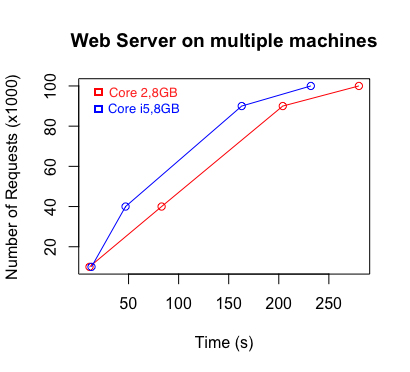
\includegraphics{Performance}
				
				\subsection{ Data Transfer Grapph }
     			  		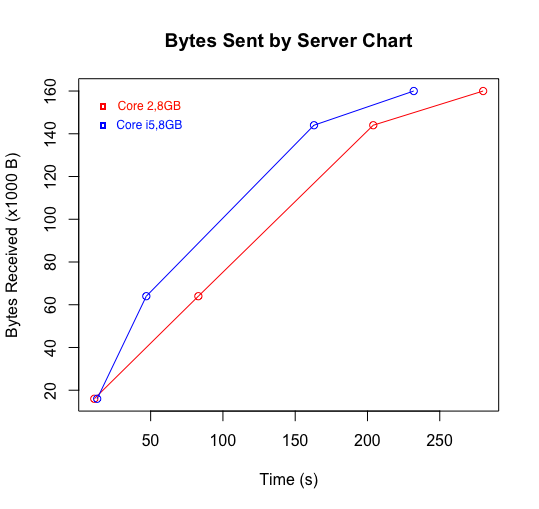
\includegraphics[scale=.75]{BytesSentGraph}
				


%\input{samplebody-journals}


\end{document}
